\section{Les revues de presse}
\label{sec:revue}

La principale fonctionnalité innovante de notre plateforme de consultation de journaux anciens est la possibilité de
créer et de partager des revues de presse.

Une revue de presse est, basiquement, une liste d'articles de journaux regroupés ensemble par un ou plusieurs utilisateurs autour d'une thématique précise,
comme par exemple une date, un événement ou une zone géographique.

L'initialisation de la revue de presse se fera de 2 façons différentes, d'abords depuis le menu principal, il y a un bouton qui permet de créer
une revue de presse vide. L'autre méthode est de cliquer sur le bouton d'ajout présent sur la page de visualisation et de cliquer
sur le bouton pour créer une nouvelle revue de presse.
la seule différence avec la premuère méthode est que la revue de presse sera initialisée avec le-dit document.

Il y aura plusieurs moyens d'ajouter un document à une revue de presse :

\begin{itemize}
  \item cliquer sur le bouton d'ajout présent sur la page de visualisation et choisir la
revue de presse à laquelle contribuer.
  \item cliquer sur le bouton d'ajout directement présent depuis le moteur de recherche et choisir
à quelle revue de presse contribuer.
  \end{itemize}

La page de visualisation d'une revue de presse serae composé du titre, de la description de la revue de presse et d'une liste comprenant les articles
de cette revue de presse. Depuis cette page il sera possible de modifier le titre, la description et de retirer un article sur cette revue de presse.
L'auteur pourra également midifier l'ordre de lecture de la revue de presse en glissant l'article à une position souhaitée.

\begin{figure}[H]
    \centering
    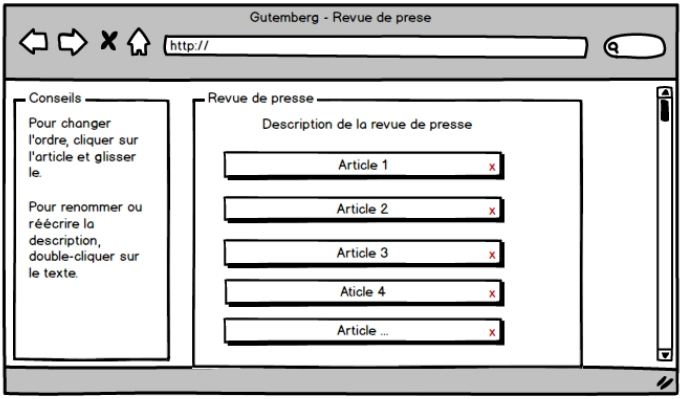
\includegraphics[width=\textwidth]{figures/revue.png}
    \caption{Page de visualisation d'une revue de presse}
    \label{fig:revue}
\end{figure}

